\documentclass{article}
\usepackage[utf8]{inputenc}

\title{Homework 6}
\author{Benny Chen}
\date{November 7, 2022}

\usepackage{color}
\usepackage{amsthm}
\usepackage{amssymb} 
\usepackage{amsmath}
\usepackage{listings}
\usepackage{listings}
\usepackage{graphicx}
\usepackage{tabularx}
\usepackage[table,xcdraw]{xcolor}
\usepackage[hidelinks]{hyperref}

\lstdefinelanguage[mips]{Assembler}{%
  % so listings can detect directives and register names
  alsoletter={.\$},
  % strings, characters, and comments
  morestring=[b]",
  morestring=[b]',
  morecomment=[l]\#,
  % instructions
  morekeywords={[1]abs,abs.d,abs.s,add,add.d,add.s,addi,addiu,addu,%
    and,andi,b,bc1f,bc1t,beq,beqz,bge,bgeu,bgez,bgezal,bgt,bgtu,%
    bgtz,ble,bleu,blez,blt,bltu,bltz,bltzal,bne,bnez,break,c.eq.d,%
    c.eq.s,c.le.d,c.le.s,c.lt.d,c.lt.s,ceil.w.d,ceil.w.s,clo,clz,%
    cvt.d.s,cvt.d.w,cvt.s.d,cvt.s.w,cvt.w.d,cvt.w.s,div,div.d,div.s,%
    divu,ecall,eret,floor.w.d,floor.w.s,j,jal,jalr,jr,l.d,l.s,la,lb,lbu,%
    ld,ldc1,lh,lhu,li,ll,lui,lw,lwc1,lwl,lwr,madd,maddu,mfc0,mfc1,%
    mfc1.d,mfhi,mflo,mov.d,mov.s,move,movf,movf.d,movf.s,movn,movn.d,%
    movn.s,movt,movt.d,movt.s,movz,movz.d,movz.s,msub,msubu,mtc0,mtc1,%
    mtc1.d,mthi,mtlo,mul,mul.d,mul.s,mulo,mulou,mult,multu,mulu,mv,neg,%
    neg.d,neg.s,negu,nop,nor,not,or,ori,rem,remu,rol,ror,round.w.d,%
    round.w.s,s.d,s.s,sb,sc,sd,sdc1,seq,sge,sgeu,sgt,sgtu,sh,sle,%
    sleu,sll,sllv,slt,slti,sltiu,sltu,sne,sqrt.d,sqrt.s,sra,srav,srl,%
    srlv,sub,sub.d,sub.s,subi,subiu,subu,sw,swc1,swl,swr,syscall,teq,%
    teqi,tge,tgei,tgeiu,tgeu,tlt,tlti,tltiu,tltu,tne,tnei,trunc.w.d,%
    trunc.w.s,ulh,ulhu,ulw,ush,usw,xor,xori},
  % assembler directives
  morekeywords={[2].align,.ascii,.asciiz,.byte,.data,.double,.extern,%
    .float,.globl,.half,.kdata,.ktext,.set,.space,.text,.word},
  % register names
  morekeywords={[3]\$0,\$1,\$2,\$3,\$4,\$5,\$6,\$7,\$8,\$9,\$10,\$11,%
    \$12,\$13,\$14,\$15,\$16,\$17,\$18,\$19,\$20,\$21,\$22,\$23,\$24,%
    \$25,\$26,\$27,\$28,\$29,\$30,\$31,%
    \$zero,\$at,\$v0,\$v1,\$a0,\$a1,\$a2,\$a3,\$t0,\$t1,\$t2,\$t3,\$t4,
    \$t5,\$t6,\$t7,\$s0,\$s1,\$s2,\$s3,\$s4,\$s5,\$s6,\$s7,\$t8,\$t9,%
    \$k0,\$k1,\$gp,\$sp,\$fp,\$ra},
}[strings,comments,keywords]

\definecolor{CommentGreen}{rgb}{0,.6,0}
\lstset{
  language=[mips]Assembler,
  escapechar=@, % include LaTeX code between `@' characters
  keepspaces,   % needed to preserve spacing with lstinline
  basicstyle=\small\ttfamily\bfseries,
  commentstyle=\color{CommentGreen},
  stringstyle=\color{cyan},
  showstringspaces=false,
  keywordstyle=[1]\color{blue},    % instructions
  keywordstyle=[2]\color{magenta}, % directives
  keywordstyle=[3]\color{red},     % registers
}

\lstdefinestyle{Python}{
    language        = Python,
    frame           = lines, 
    basicstyle      = \footnotesize,
    keywordstyle    = \color{blue},
    stringstyle     = \color{green},
    commentstyle    = \color{red}\ttfamily
}

\begin{document}

\maketitle

\section*{Problem 1}
Assume the single-cycle RISC-V processor, as shown in Figure 4.21. Find the following
signal values when the processor executes the instruction 0xFE542023 located at
0x00400200. Explain your answers.
All signals generated by the main control. \\\\
Instruction: 0x00400200 : 0xFE542023 \\
Binary: 010000000000001000000000 : 1111111 00101 01000 010 00000 0100011
\begin{itemize}
    \item opcode: instruction[6:0] = 0100011 = 0x23
    \item rs1: instruction[19:15] = 01000 = 0x8
    \item rs2: instruction[24:20] = 00101 = 0x5
    \item rd: instruction[11:7] = 00000 = 0x0
    \item Immediate: instruction[11:5, 4:0] = 1111 1110 0000 extended to 32 bits = 0xFFFFFFE0
    \item ALU operation: 0010
    \item BranchTarget: 0x00400200 + 0xFFFFFFE0 = 0x004001E0
    \item PCSrc: 0
    \item NextPC: 0x00400200 + 4 = 0x00400204
\end{itemize}
\newpage

\section*{Problem 2}
a.
\begin{center}
    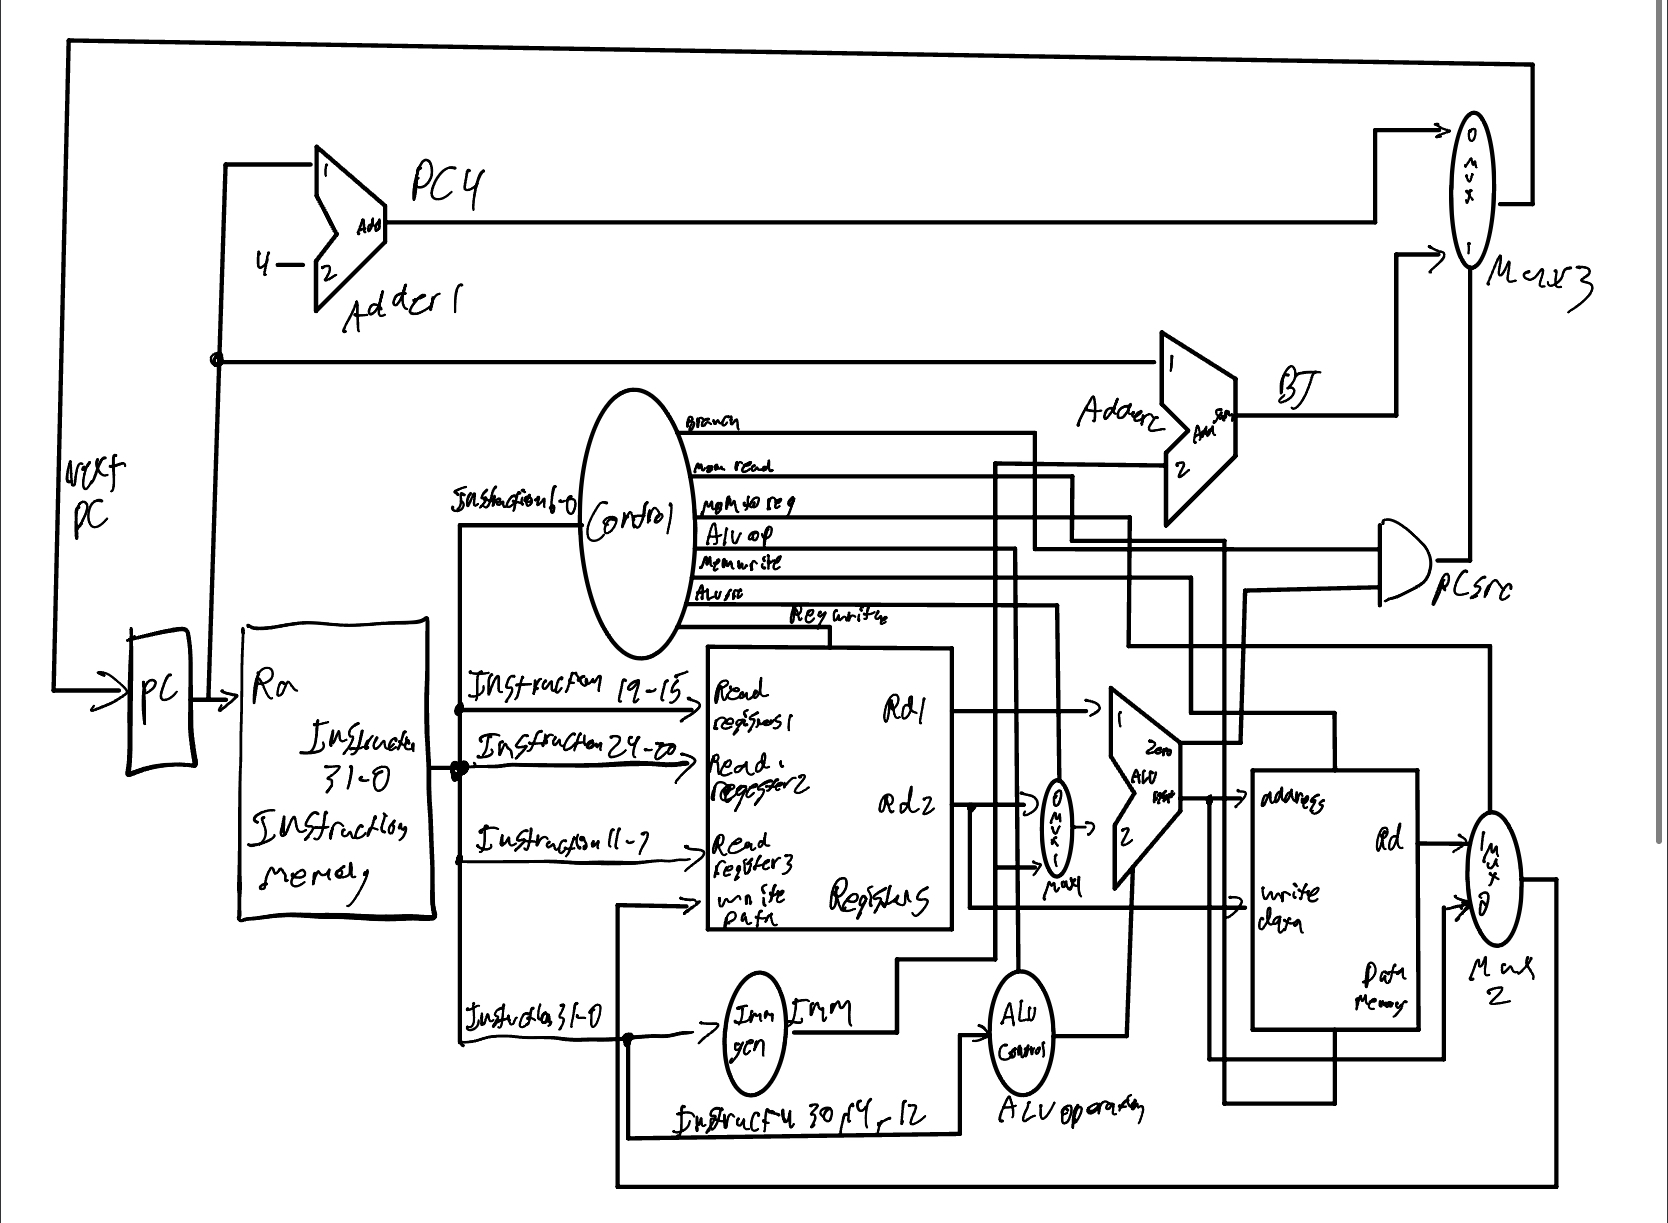
\includegraphics[scale=.19]{./images/normal.png}
\end{center}

b.
\begin{center}
    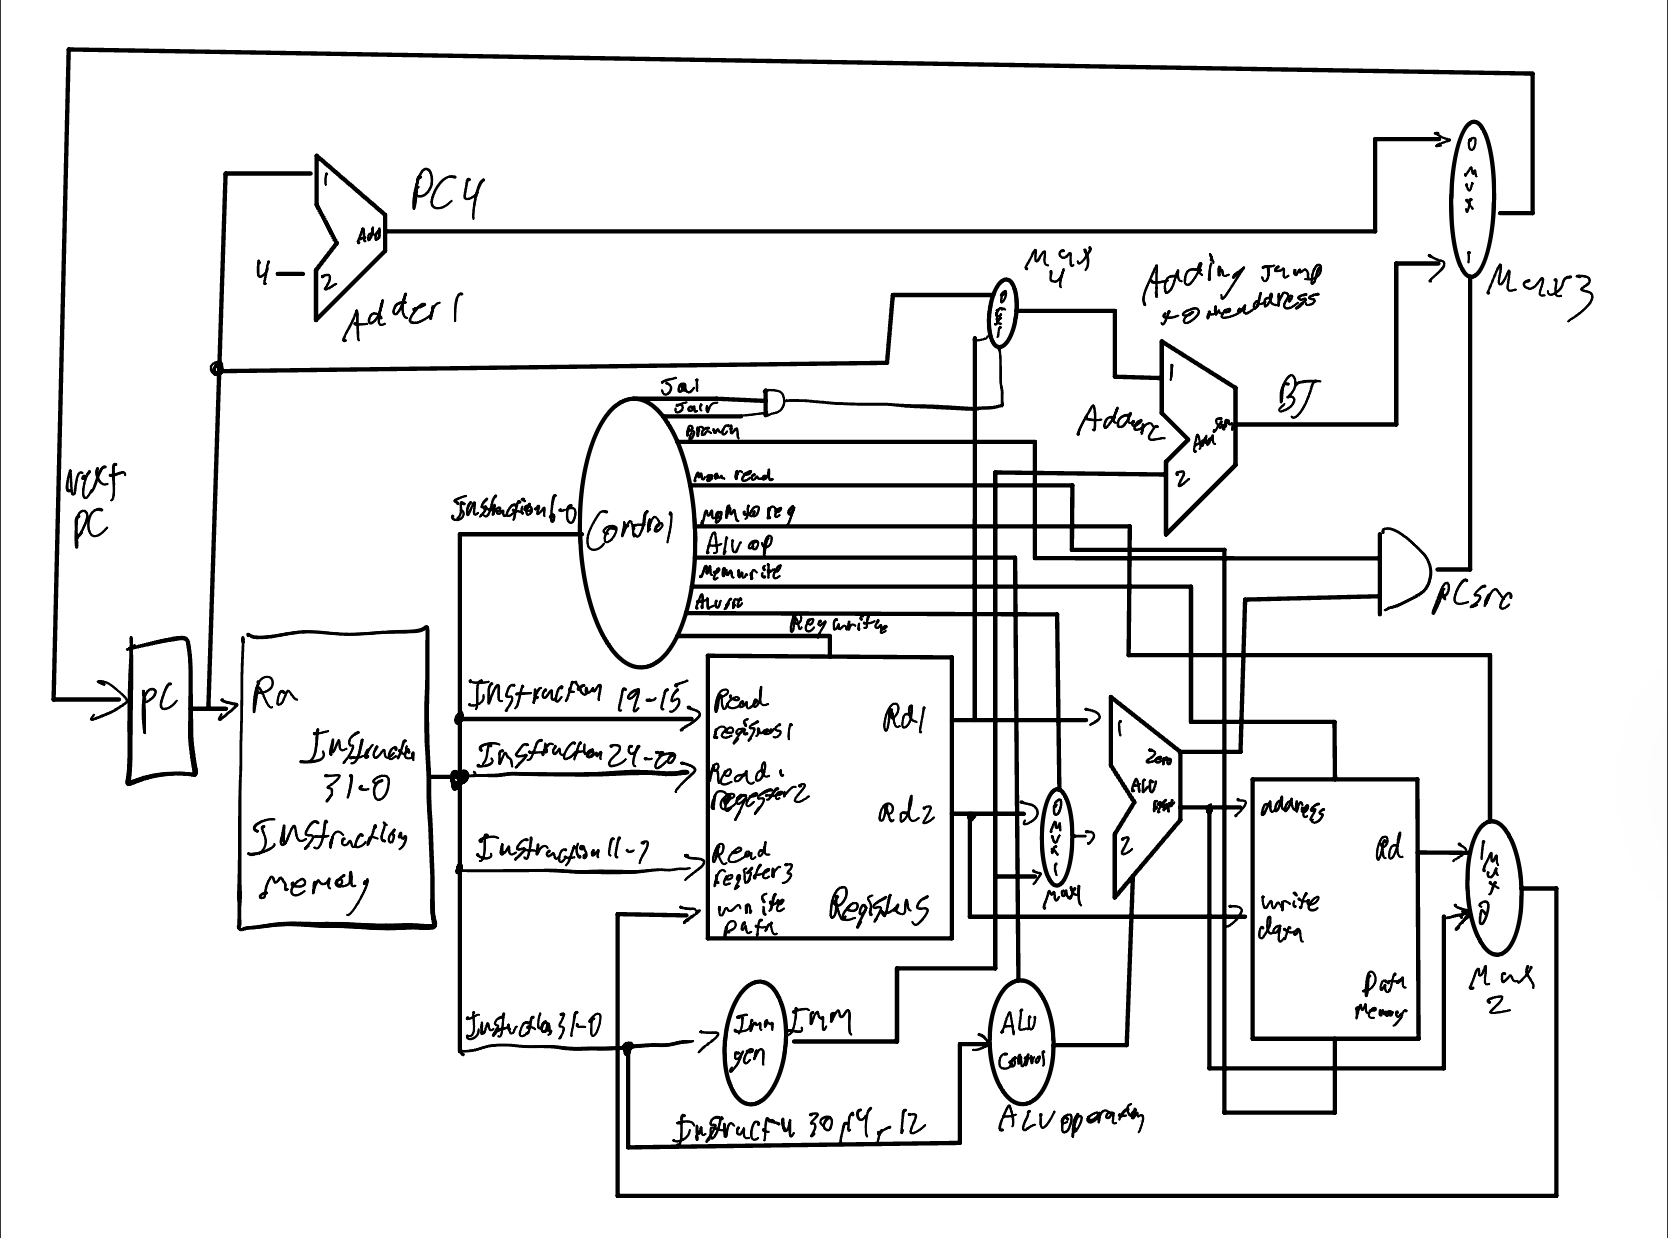
\includegraphics[scale=.19]{./images/a.png}
\end{center}
JAL: PC + Immediate
JALR: RD (Read Data) + immediate
c.
\begin{center}
    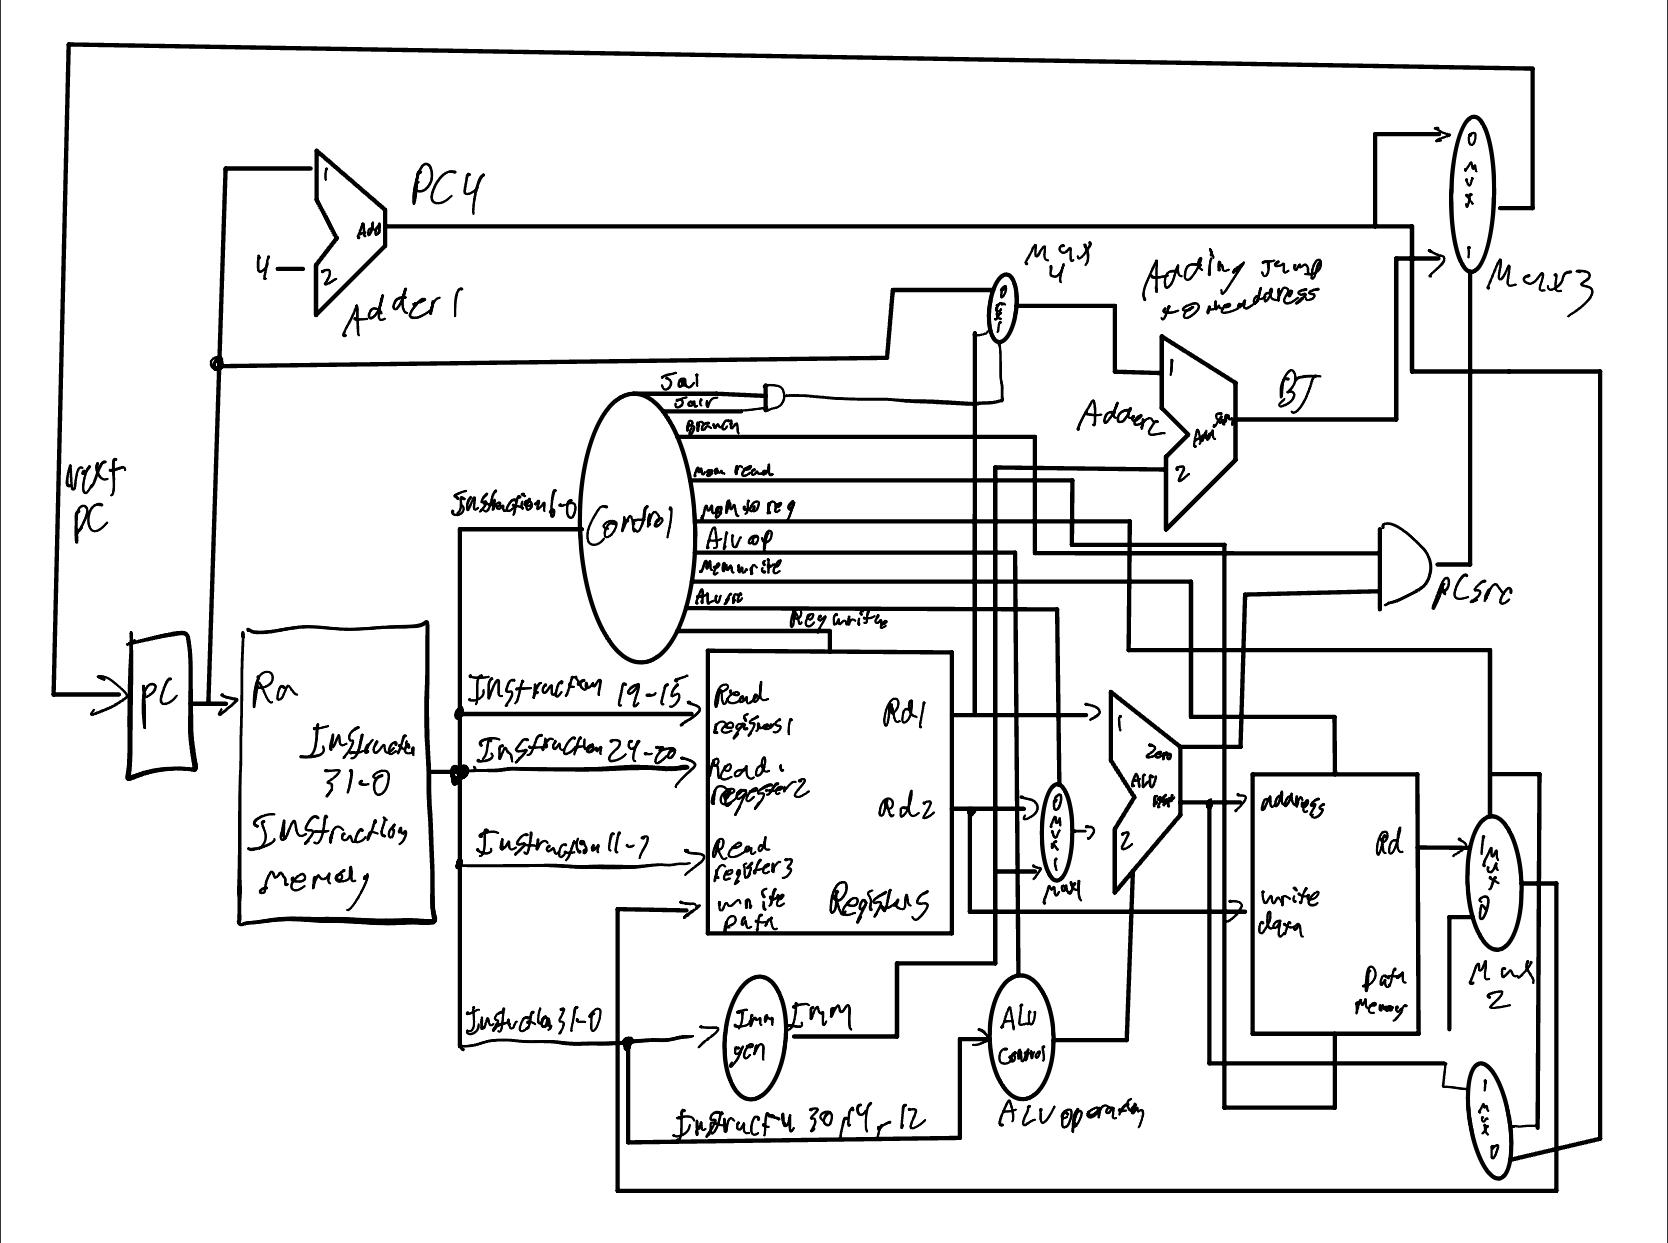
\includegraphics[scale=.19]{./images/b.png}
\end{center}
d.
\begin{table}[h]
    \resizebox{\textwidth}{!}{%
    \begin{tabular}{|l|r|r|l|l|l|l|l|l|}
    \hline
    Inst.                       & \multicolumn{1}{l|}{ALU Src} & \multicolumn{1}{l|}{Memto Reg} & Reg Write & Mem Read & Mem Write & Branch & J & JR \\ \hline
    \cellcolor[HTML]{FFFFFF}JAL & X                            & 0                              & 1         & 0        & 0         & 0      & 1 & 0  \\ \hline
    JALR                        & X                            & 0                              & 1         & 0        & 0         & 0      & 1 & 1  \\ \hline
    \end{tabular}%
    }
\end{table}




\end{document}